\subsection{Security Enclaves}

A security enclave is a group of nodes that follow the same security policy. Enclaves usage are specified upon execution time, implying that their security artifacts are actually used by running processes.

Typically, a node is perceived as an abstraction of a DDS \textit{participant}. However, by considering node composition, as a reliable way for matching multiple nodes simultaneously to the same enclave, this node perception as participants can not be taken into account, due to causing non-negligible overhead. There is also not convenient to compose nodes as individual participants, as far as operating system's security is concerned, where permission distribution and memory becomes rather difficult to handle. \cite{ros-security-enclaves, ros-access-control}

To address this, each participant must be matched to a node shared context, instead of being directly related to a specific node. Thereby, the initial given definition of an enclave is not totally correct, since a participant can either be perceived as single node or as multiple node shared context. So, each enclave security artifacts are used by its respective DDS participant. \cite{ros-security-enclaves}

\subsection{Access Control}

To properly introduce the set of tools that SROS2 provides, it follows an application example that will now account the security features, as to provide authentication and encryption over the network communication, as well as access control policies over the application nodes. 

\subsubsection{The \textit{TurtleSim} Application}

For instance, consider a well-known example called \textit{TurtleSim}, which is a simulator typically used for learning ROS, mainly composed by \textit{two nodes}, that perform together towards moving a turtle. Additional nodes were implemented, in order to add complexity to the current network, as to later support security as a proper example.

For understanding reasons, the reader may want to see how the network architecture is organized. ROS2 provides a GUI tool called \textit{rqt}, that assists developers in manipulating the network elements, in a more user-friendly manner. The \textit{rqt} visualizer, \textit{rqt\_graph}, allows the developer to perform analysis over a graphical visualization of the network computation graph.

\begin{figure}[H]
    \centering
    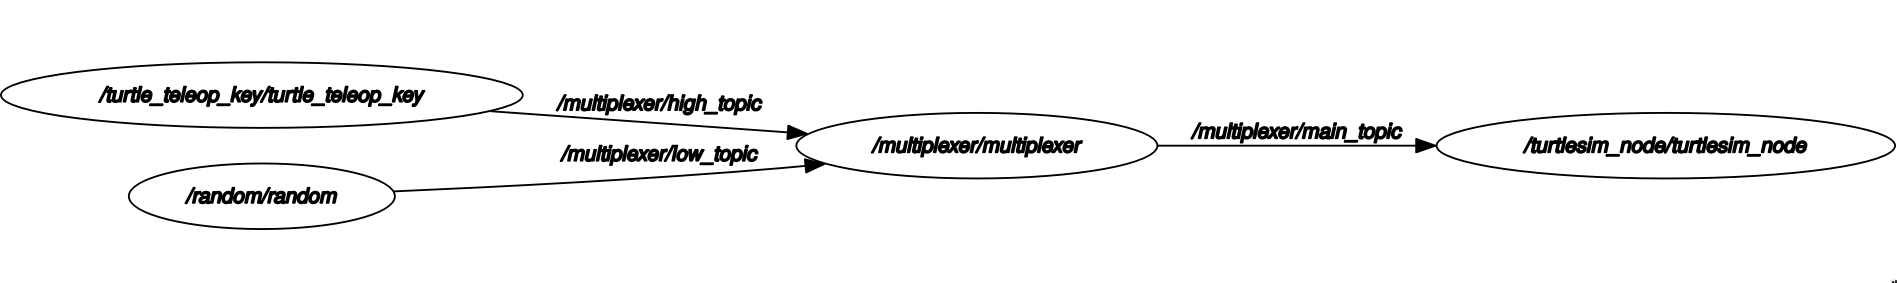
\includegraphics[width=0.8\linewidth]{images/ts_rqt_graph.png}
    \caption{\textit{TurtleSim}'s network graph presented by \textit{rqt\_graph}.}
    \label{fig:ts-rqt-graph}
\end{figure}

The \textit{multiplexer} node handles commands related to turtle's movement, acting as a topic selector between two different subscribed topics, each of them was respectively associated with a priority value. Based on the priority valued, the \textit{multiplexer} node forwards the commands, related to the selected topic, into the \textit{turtlesim} node, triggering the turtle's movement. 

However, \textit{multiplexer} is not exclusive to the \textit{turtlesim} node, as it is still possible to directly publish commands to the topic that handles the turtle's movement, since security policies are yet to be implemented.

\subsubsection{Application Configuration}

To accurately achieve topic exclusivity, in which the turtle's movement is uniquely concerned by the \textit{multiplexer} node, \textit{access control} policies must be applied. The remaining nodes should be considered untrustworthy, denying any potential undesired turtle's movement.
            
In order to provide access control, each permission file needs to be modified, accounting the network policies restrictions. This is ensured by adding security permissions to these files, with the mandatory signature of the Certificate Authority. A suitable way of editing the permission file, \textit{permissions.xml} (file that dictates how the enclave manages the permissions within the network) is by creating a policy file, that explicitly specifies the set of permissions of each enclave.

Following the \textit{ConArmor} policy language \cite{white2018procedurally}, the \textit{SROS2 policy file} confers a restrict \textit{XML schema}, where security policies bind profiles to access permissions for network objects, granting privileges back to a certain profile. \textit{Profiles} are implemented under the \textit{enclave} declaration, to duly support the node composition into a single process, enabling the possibility of combining multiple profiles, respectively addressing its corresponding node. Typically, each \textit{enclave} declaration is linked to a corresponding ROS node, naturally perceived as a DDS participant.

\textit{Objects} are classified over a subsystem type, structurally characterized by permissions tags. Then \textit{object privileges} are controlled over access values, either \textit{allow} or \textit{deny}, attributed to their corresponding permissions tags. For instance, consider the \textit{topics} domain, where a profile can either publish or subscribe to that topic. To properly address the allowance of a profile privilege over a topic, the permission tag (either subscribe or publish) must be followed with the \textit{allow} tag. \cite{ros-access-control}

The policy design approach works under the \textit{Mandatory Access Control} (MAC), that denies any privilege by default. The only way of allowing access to any object, is by explicitly specifying the subject's privilege access. \cite{ros-access-control, white2018procedurally}

In technically terms, a \textit{keystore} must be initiated beforehand, to provide a secured environment over the network. SROS2 yields a command that permits its creation. A keystore is a created directory where files regarding security are stored. By generating a keystore directory, it may then be sourced and utilized by \textit{rcl} features towards applying security to the application. The \textit{security} additional keyword-flag enables features regarding security matters, concerning the DDS-security artifacts.
            
\begin{lstlisting}[title={\textit{Keystore} creation using the proper SROS2 command.}]
ros2 security create_keystore demo
\end{lstlisting}

Upon the creation of the \textit{demo} keystore, three respective subdirectories are created, where each has their own role when it comes to security enhancement over the network.

\textbullet\  The \textit{enclaves} directory contains the security tools related to each enclave created. An \textit{enclave} is a group of ROS nodes, controlled by the same set of security rules, defined in its corresponding enclave directory.

\textbullet\  The \textit{public} directory contains material that is permissible as public. A Certificate Authority certificate is stored in this directory, related to the CA \textit{public key}. It is used to validate the identity and permissions of each ROS network node by the CA. 

\textbullet\  The \textit{private} directory contains material that is considered private. A Certificate Authority certificate is stored in this directory, related to the CA \textit{private key}. It is used to modify the network policies, such as access permissions, and to add new participants. Similar to the public directory, the CA key corresponding to its identity and permissions can be stored in their corresponding individual directories.

The following exports need to be sourced to force SROS2 security features, as they concern relevant environment variables. The first sourced variable points to the directory root of the keystore, allowing ROS2 to identify where the security artifacts are kept. The second serves as the security enabler. The last variable sets which security strategy will be used when dealing with security files.
            
\begin{lstlisting}[title={SROS2 environment variables.}]
export ROS_SECURITY_KEYSTORE=/demo
export ROS_SECURITY_ENABLE=true
export ROS_SECURITY_STRATEGY=Enforce
\end{lstlisting}
            
\subsection{Understanding Security Enclaves}

Once the keystore has been created, the respective enclaves can be implemented. As mentioned, an enclave is a group of nodes that follow the same security policy. Enclaves usage are specified upon execution time, implying that their security artifacts are actually used by running processes.

Typically, a node is perceived as an abstraction of a DDS \textit{participant}. However, by considering node composition, as a reliable way for matching multiple nodes simultaneously to the same enclave, this node perception as participants can not be taken into account, due to causing non-negligible overhead. There is also not convenient to compose nodes as individual participants, as far as operating system's security is concerned, where permission distribution and memory becomes rather difficult to handle. \cite{ros-security-enclaves, ros-access-control}

To address this, each participant must be matched to a node shared context, instead of being directly related to a specific node. Thereby, the initial given definition of an enclave is not totally correct, since a participant can either be perceived as single node or as multiple node shared context. So, each enclave security artifacts are used by its respective DDS participant. \cite{ros-security-enclaves}

As long as security is enabled, the whole network must be properly authenticated. Thus, every node within the network must be authenticated, using an enclave as their identifier. Node composition can not be considered in this network, as it is not intended to share topic privileges. Note that, if an enclave was shared by multiple nodes, each node policy would be considered as common policy within the enclave. \cite{ros-access-control}

\begin{lstlisting}[title={\textit{TurtleSim} enclave creation.}]
ros2 security create_key demo /turtlesim
ros2 security create_key demo /multiplexer
ros2 security create_key demo /keyboard
ros2 security create_key demo /random
\end{lstlisting}

The keystore creation, alongside with their respective enclaves, only ensures security over the network communication, in which node authentication and data encryption are concerned. With the proper use of port scanning tools, data encryption can be easily verified. Authentication is ensured upon the enclave's creation. However, to properly apply security over the \textit{TurtleSim} application, access control policies must be appropriately covered.

\subsubsection{Access Control}

To accurately achieve topic exclusivity, in which the turtle's movement is uniquely concerned by the \textit{multiplexer} node, \textit{access control} policies must be applied. The remaining nodes should be considered untrustworthy, denying any potential undesired turtle's movement.
            
In order to provide access control, each permission file needs to be modified, accounting the network policies restrictions. This is ensured by adding security permissions to these files, with the mandatory signature of the Certificate Authority. A suitable way of editing the permission file, \textit{permissions.xml} (file that dictates how the enclave manages the permissions within the network) is by creating a policy file, that explicitly specifies the set of permissions of each enclave.

Following the \textit{ConArmor} policy language \cite{white2018procedurally}, the \textit{SROS2 policy file} confers a restrict \textit{XML schema}, where security policies bind profiles to access permissions for network objects, granting privileges back to a certain profile. \textit{Profiles} are implemented under the \textit{enclave} declaration, to duly support the node composition into a single process, enabling the possibility of combining multiple profiles, respectively addressing its corresponding node. Typically, each \textit{enclave} declaration is linked to a corresponding ROS node, naturally perceived as a DDS participant.

\textit{Objects} are classified over a subsystem type, structurally characterized by permissions tags. Then \textit{object privileges} are controlled over access values, either \textit{allow} or \textit{deny}, attributed to their corresponding permissions tags. For instance, consider the \textit{topics} domain, where a profile can either publish or subscribe to that topic. To properly address the allowance of a profile privilege over a topic, the permission tag (either subscribe or publish) must be followed with the \textit{allow} tag. \cite{ros-access-control}

The policy design approach works under the \textit{Mandatory Access Control} (MAC), that denies any privilege by default. The only way of allowing access to any object, is by explicitly specifying the subject's privilege access. \cite{ros-access-control, white2018procedurally}

\begin{lstlisting}[title={Setting permissions into each enclave.}]
ros2 security create_permission demo /turtlesim policies.xml
ros2 security create_permission demo /multiplexer policies.xml
ros2 security create_permission demo /keyboard policies.xml
ros2 security create_permission demo /random policies.xml
\end{lstlisting}

As it follows, security is enabled within this network as well as policy control over topic's permissions. The network can be easily configured and automatically launched through the execution of a launch file, where \textit{roslaunch} uses this files to perform overall initialization.

\begin{figure}[H]
\begin{lstlisting}
<launch>
    <node name="turtlesim" pkg="default" exec="turtlesim" output="screen" args="--ros-args --enclave /turtlesim" />
    <node name="keyboard" pkg="default" exec="keyboard" output="screen" args="--ros-args --enclave /keyboard" />
    <node name="random" pkg="random" exec="random" args="--ros-args --enclave /random" />
    <node name="multiplexer" pkg="multiplexer" exec="multiplexer" args="--ros-args --enclave /multiplexer" />
</launch>
\end{lstlisting}
\caption{\textit{TurtleSim} launch file.}
\label{fig:ros-lf}
\end{figure}

The network is now sucessfully running as a secured environment, where nodes within this network can not be perceived from outside, neither their topic list. To prove that access control is properly employed, the user may want to try to enhance the turtle movement directly from the random controller, by forcing the remapping of the \textit{low\_topic} to the \textit{main\_topic}. Thus, by attempting to remap the \textit{low\_topic} topic prevents the node from launching, since the random node is only allowed to publish through the \textit{low\_topic}. 

\begin{lstlisting}[title={Attempting the \textit{low\_topic} remap.}, language=xml]
<node name="random" pkg="turtle_random" exec="random" args="--ros-args --enclave /random -r /low_topic:=/main_topic"/>
\end{lstlisting}

% However, if the user forces the inverted remap, it is possible to control the turtle movement directly from the random controller, since no policie has been disrespecteded. Although, the random controller is still publishing to the \textit{low\_topic}, the \textit{main\_topic} in which the turtle movement is concerned is remapped towards the \textit{low\_topic}. This concerns a problem that is not been duly address by the ROS community. It is unreasonable to expect this flexibility in a secured network, since policies initially settled can be easily compromised.